\chapter{Marco Teórico}
En el presente capítulo se definen las bases teóricas sobre las cuáles se apoya el proyecto. Para el desarrollo de la aplicación \textit{CPI} se utilizó Umbraco \cite{umbraco} como plataforma principal para manejo de contenido (CMS) \cite{cmsBarker} y se usó el patrón MVC \cite{mvcKrasner}.

\section{Bases Teóricas}

\subsection{CMS}
Un Sistema de Gestión de Contenido o CMS, por sus siglas en inglés \textit{Content Management System}, es un paquete de software que brinda cierto nivel de automatización de las tareas requeridas para administrar el contenido de manera efectiva. Un CMS permite a los usuarios crear nuevo contenido, editar contenido existente, y hacer el contenido accesible al público \cite{cmsBarker}.

Para los editores, el CMS les permite crear contenido nuevo, editar contenido existente, realizar procesos con el contenido mediante una interfaz de edición (referida como \textit{back-end} que es la capa de acceso a los datos de la aplicación) y finalmente les permite colocar este contenido a disposición de otros usuarios en una interfaz (referida como el \textit{front-end}, es decir, la capa de presentación de la aplicación).

Un CMS permite el control del contenido, esto se refiere a que mantiene un constante seguimiento del contenido (donde se encuentra el contenido, quién puede acceder a él, y cómo se relaciona con otros contenidos). Por otro lado permite la reutilización del contenido (usar contenido en más de un lugar).

Una de las mayores ventajas del uso de CMS es que facilita las tareas mencionadas anteriormente para usuarios que no tienen preparación técnica. En el caso de la aplicación \textit{CPI}, la mayoría de los usuarios no poseen conocimientos especializados en el área de computación, por lo cual es conveniente el desarrollo del sistema sobre un CMS

El CMS sobre el cual se trabajó para el desarrollo de la aplicación cuenta con funcionalidades que ya están implementadas que son necesarias para ésta, como la autenticación para los usuarios, permisología, interfaces que facilitan el manejo de la base de datos, entre otras cosas. Cuenta con gran variedad de paquetes, librerías y módulos que facilitan el desarrollo de la aplicación.

\subsection{Modelo Cliente-Servidor}
Arquitectura de redes de computadoras ampliamente utilizado y que forma la base del uso de redes en gran medida, consta de dos entidades: un cliente y un servidor. El cliente le envía una solicitud al servidor y espera una respuesta. Luego, el servidor recibe la solicitud, lleva a cabo el trabajo requerido, o busca los datos solicitados y devuelve una respuesta al cliente \cite{redesTanenbaum}.

El servidor mantiene una relación de uno-a-muchos con los clientes, por otro lado ambos términos pueden ser vistos como “roles”, pues es posible que una máquina o proceso ejecute labores tanto de cliente como de servidor (por ejemplo, un servidor puede enviar una petición a otro servidor, si el mismo carece de los recursos que le fueron solicitados, convirtiéndose así en un cliente). Es importante destacar que los términos “cliente” y “servidor” pueden referirse tanto a máquinas como a programas o procesos. Esta arquitectura es ampliamente utilizada en aplicaciones web.

\subsection{MVC}
MVC, siglas para Modelo-Vista-Controlador, es un patrón de software utilizado ampliamente en la actualidad. Consiste en separar los datos de la aplicación (Modelo), la interfaz con el usuario (Vista), y la lógica de control (Controlador) en tres componentes distintos. Al realizar esta separación se reduce la complejidad del diseño arquitectónico y se incrementa la flexibilidad, la reusabilidad y mantenimiento del código. Adicionalmente, se pueden realizar cambios sobre un componente sin afectar a los demás, lo cual permite que cada componente tenga ciclos de desarrollo independientes del resto \cite{mvcKrasner}. 

Cabe destacar que este patrón es usado frecuentemente en el desarrollo de aplicaciones web, por lo que resulta bastante sencillo aplicarlo al modelo cliente-servidor utilizado en la aplicación. \textit{CPI} fue desarrollado usando una plataforma de desarrollo web basada en .NET \cite{netMicrosoft} que implementa este patrón.

\subsection{API}
Un API, llamado así por sus siglas en inglés para \textit{Application Programming Interface} (Interfaz de Programación de Aplicaciones), es un conjunto de comandos, funciones, protocolos y objetos que permiten exponer los datos de una aplicación de software, establecen las reglas y los mecanismos a través de los cuales se puede tener acceso a estos datos. También permite la interacción con algún software externo \cite{apiChristensson}.

El API sirve como intermediario entre dos aplicaciones, por ejemplo una aplicación dispone del API de otra para obtener los datos que se encuentran en la última y usarlos para proveer algún servicio a sus usuarios. En el caso de \textit{CPI} se desarrolló un API para poder acceder a datos de la aplicación.

\subsection{Servicio Web} \label{WebService}
Un servicio web es una aplicación o fuente de datos a la que se puede acceder a través de un protocolo web estándar, diseñado para soportar interacción máquina-máquina a través de una red, proveen una vía estándar para la comunicación entre distintas aplicaciones de software ejecutadas en distintas plataformas y ambientes. La mayoría de los servicios web proporcionan un API, para que se puedan acceder a los datos \cite{webServiceChristensson}.

Para la aplicación \textit{CPI} en el desarrollo se incluyó un módulo de servicios web, el cual permite el acceso a datos de la aplicación.

\subsection{REST}
Transferencia de Estado Representacional o REST, por sus siglas en inglés, es un estilo de arquitectura para sistemas de hipermedia distribuidos (como la \textit{World Wide Web} o red informática mundial) que define una serie de restricciones que, cuando se aplican en conjunto, enfatizan la escalabilidad de interacciones entre componentes, la generalidad de las interfaces y el despliegue independiente de componentes \cite{restFielding}.

Las restricciones definidas para los sistemas REST son las siguientes:

\begin{enumerate}
   \item \textbf{Separación Cliente-Servidor} el cliente y el servidor actúan independientemente, la interacción entre ellos ocurre solo a través de solicitudes que realiza el cliente, y las respuestas que envía el servidor como una reacción a una solicitud. El servidor solo envía información cuando ésta es solicitada por algún cliente.
   \item \textbf{Sin estado (\emph{stateless} en inglés)} el servidor no guarda información de ningún usuario que use los servicios del sistema. Cada solicitud individual contiene toda la información necesaria para ser ejecutada y enviar una respuesta, independientemente de todas las demás solicitudes que sean atendidas.
   \item \textbf{Permite el uso de memoria caché} la respuesta debe estar explícita o implícitamente etiquetada como \textit{cacheable} (se puede guardar en alguna memoria caché) o \textit{non-cacheable} (no se puede guardar en ninguna memoria caché). La ventaja del uso de memoria caché es que se pueden eliminar parcial o completamente algunas interacciones mejorando así el rendimiento del sistema.
   \item \textbf{Interfaz uniforme} cada solicitud al servidor debe tener los mismos componentes:
        \begin{itemize}
            \item Identificador del recurso deseado (en el caso de aplicaciones web este identificador puede ser el URL).
            \item Respuesta del servidor que debe incluir suficiente información para que el cliente pueda modificar el recurso (la información necesaria para que el servidor pueda llevar a cabo la solicitud y toda respuesta del servidor debe tener la información necesaria para que el cliente la entienda.
            \item Usar hipermedia como motor del estado de la aplicación, lo que quiere decir que el servidor debe poder informar al cliente las formas en las que puede cambiar el estado de la aplicación a través de enlaces de hipermedia, una página web específica se puede considerar un estado de la aplicación y enlaces incluidos en esa página se consideran transiciones a otros estados de la aplicación.
        \end{itemize}
    \item \textbf{Sistema por capas} entre el cliente que realiza una solicitud y el servidor que envía la respuesta final puede haber varios servidores, por ejemplo, puede haber un servidor que proporcione una capa de seguridad, otro una capa de memoria caché, y otros con otras funcionalidades. Estos servidores intermedios no deben afectar ni la solicitud ni la respuesta. Además, cada transacción (envío de la solicitud por el cliente y la subsiguiente respuesta) debe ser transparente para el cliente, es decir, el cliente no tiene conocimiento de las capas intermedias por las que pasan la solicitud y la respuesta.
\end{enumerate}

Se dice que un servicio web o el API de un servicio web es \textit{RESTful} cuando cumple con todas estas restricciones. El proyecto presente se desarrolló adhiriéndose a estas restricciones.

\subsection{SaaS}

Un Software como Servicio o SaaS, por sus siglas en inglés \textit{Software as a Service}, es un modelo para la distribución de software donde los clientes acceden al software a través de Internet. En SaaS, un proveedor de servicios aloja la aplicación en su centro de datos y un cliente accede a ella a través de un navegador web estándar \cite{saas}.

\subsection{Modelo "4+1" de Kruchten}

El modelo “4+1” de Kruchten, es un modelo de vistas diseñado por el profesor Philippe Kruchten y que encaja con el estándar “IEEE 1471-2000” que se utiliza para describir la arquitectura de un sistema software intensivo basado en el uso de múltiples vistas que deben estar relacionadas entre sí (ver Figura \ref{fig:vistas}) \cite{vistasKruchten}. Cada una de estas vistas permite abordar por separado las inquietudes de los distintos "interesados" de la arquitectura: usuario final, desarrolladores, ingenieros de sistemas, gerentes de proyectos, entre otros, y manejar por separado los requisitos funcionales y no funcionales. Las vistas que abarca este modelo son:
\begin{itemize}
	\item Vista Lógica: En esta vista se representa la funcionalidad que el sistema proporciona a los usuarios finales, es decir, se ha de representar lo que el sistema debe hacer y las funciones y servicios que ofrece.
	\item Vista de Despliegue: En esta vista se muestra el sistema desde la perspectiva de un programador y se ocupa de la gestión del software, es decir, se muestra como esta dividido el sistema de software en componentes y las dependencias que hay entre estos componentes.
 	\item Vista de Procesos: En esta vista se muestran los procesos que hay en el sistema y la forma en la que se comunican estos procesos, se muestra desde la perspectiva de un integrador de sistemas, el flujo de trabajo paso a paso de negocio y operaciones de los componentes que conforman el sistema.
	\item Vista Física: Se muestra desde la perspectiva de un ingeniero de sistemas todos los componentes físicos del sistema, así como las conexiones físicas entre esos componentes que conforman la solución.
	\item Vista de Escenarios: Esta vista va a ser representada por los casos de uso  software y va a tener la función de unir y relacionar las otras 4 vistas.
\end{itemize}

\begin{figure}[H]
    \begin{center}
    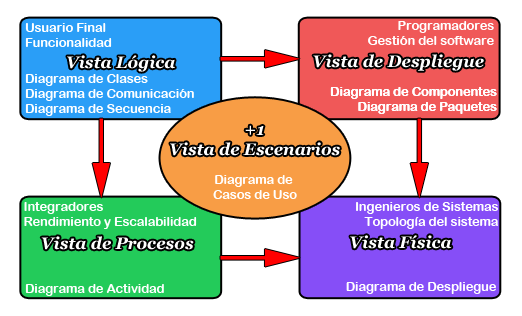
\includegraphics[width=\textwidth]{vistas.png}
    \caption{Modelo “4+1” de Kruchten}
    \label{fig:vistas}
    \end{center}
\end{figure}

\subsection{Document type (Doctype)}
Un Document Type es la definición de datos para el contenido de un sitio web, es el concepto mas importante de Umbraco. Es un concepto análogo a la definición de una clase en un lenguaje orientado a objetos, no son el contenido o datos sino la definicion de su estructura y propiedades. 
\subsection{Data type}
Un Data Type determina la estructura y el tipo de información que puede ir en una propiedad de un Doctype.
\subsection{Back Office}
Se entinde por Back Office al back end de Umbraco, la interfaz de administración de contenido de un sitio de Umbraco, se accede a el mediante una ruta especial y es necesario poseer credenciales para poder ingresar. El back office se divide en secciones, las cuales por defecto son: Content (para gestión de contenido), Media (gestión de archivos multimedia), Settings (gestión de los Document Types del sitio, plantillas del front end, scripts, idiomas, diccionario y los tipos de archivos multimedia), Developer (gestión de paquetes, macros y Data Types), Users (gestión de usuarios con credenciales para entrar al back office) y Members (gestión de usuarios con credenciales al front end).
\subsection{Nodo} \label{nodoUmbraco}
El contenido de Umbraco se guarda como nodos en un árbol de contenidos. Cada nodo es una instancia de un Doctype.
